%% ----------------------------------------------------------------
%% Conclusion.tex
%% ---------------------------------------------------------------- 
\chapter{Conclusion and Future Work} \label{Chapter: Conclusion}
This thesis studied the apple detection problem, in the context of general fruit detection using, a deep learning-based algorithm, RetinaNet. Previous works have demonstrated repeatedly the superiority of deep learning-based methods for agricultural purposes, especially in the field of fruit detection. The biggest advantage of deep learning is that it entirely dismissed feature engineering, which requires expertise from the domain knowledge; thus it enabled the development of algorithms that apply in universal datasets instead of being crop-specific.

RetinaNet, exploits the pyramidal feature hierarchy of the backbone network to build higher level semantic maps. From each intermediate backbone layer it obtains feature maps of different spatial sizes, each containing different levels of information. Combining coarse feature maps, rich in information, with spatially larger semantically weak maps, results in finer maps, containing large amounts of information. The resulting feature maps, are five pyramidal levels of increasing resolution, each with high content in semantic information, enabling detection in multiple scales.

Despite that the hyper-parameter tuning is essential for efficient optimisation, recent work in fruit detection has not given the necessary attention. In this specific study, the right predefined anchor boxes' sizes, have been configured efficiently, through an evolution search algorithm, enabling easier regression. Furthermore, loss has been modified to take more stable values, accelerating convergence. Moreover, an analysis between the dataset's annotation size distribution and the predictions' sizes from each pyramidal level of RetinaNet, showed that possibly some layers might be redundant advocating a deeper exploration in alternative, simpler architectures, thus, side-network's efficiency was studied through four proposed alternative deployments.

Concerning network's effectiveness, it was demonstrated that performance scales with the depth of the backbone network, however, that was not the case with the side-network. The lightweight RetinaNet - $\text{C}_\text{i}\text{Reduced}$ consistently performed better comparing to more sophisticated architectures, proving that by semantically enriching the feature maps, or increasing side-network's complexity in a different manner, does not help this binary problem.

Afterwards, an investigation between performance and training size relation, showed that even 10 samples are enough for adequate detection. Moreover, maximum performance could be achieved by using only 200-500 samples (at least 2x times less than the original training set) relieving growers from labelling big datasets. This finding raises questions around the dataset, as deep learning algorithms, generally, perform better as the training dataset increases.

In the last section, optimisation for peak detection demonstrated that, indeed, high resolutions yield better results, but with infinitesimal difference. However, increasing resolution, increases training and inference time as well. RetinaNet - $\text{C}_\text{i}\text{Reduced}$(VGG16) reached the maximum performance of AP=\textbf{0.955} and F1=\textbf{0.908} using a resolution of $800\times1220$ outperforming the state-of-the-art (\cite{bargoti2017deep}). The same model trained on dataset's original resolution ($202\times308$), achieved an AP=\textbf{0.948} and an F1-score=\textbf{0.895} with detections rate of \textbf{69.5} FPS, x1.5 times faster than the model of \cite{liang2018apple}. Furthermore, the model managed to maintain its first-rate performance even under the more strict $\text{IoU}_{th}$ of 0.5.

Concerning model's limitations, as shown in \sref{nms_threshold}, the detector suppresses detections with overlap $\text{IoU}\geq\text{NMS}_{th}$, as these predictions are registered as multiple detections (Figures \ref{fig4_2}, \ref{fig4_3} and \ref{ch4:fig6}). However, the severity of this problem depends on the context of the application, the framework has been implemented into; e.g. for robotic harvesting it is not very crucial, as after a fruit has been gathered, the algorithm can update the detected instances through a new image, while for yield estimation applications it is harmful, as the model will always undercount. Furthermore, acquiring data with monocular cameras make the model prone to double counting, as the model does not identify the objects across  frames; thus, farmers should put extra effort obtaining datasets with unique instances. Lastly, monocular RGB cameras are incapable of estimating depth, thus the model struggles distinguishing between foreground and background (\fref{fig3}) resulting in learning spurious rules such as classifying relevant objects by their relative size.

The ACFR dataset consists of crops of images that span entire trees in an orchard block. The proposed technique can be commercialised through a robotic harvesting application from unmanned ground vehicles, as it allows accurate detections from images captured in relatively short distances. As future work, it is left to explore algorithm's full potential in real-time detections, such as equipped on drones flying between orchard rows. This can be studied through sequential images of entire trees without sub-sampling, to investigate if the state-of-the-art performance can be preserved in samples with smaller fruits. Integrating tracking designs on the system such as the Hungarian Algorithm, can provide accurate yield mappings.


 \begin{figure}[!ht]
  \centering
  \subfigure[]{
    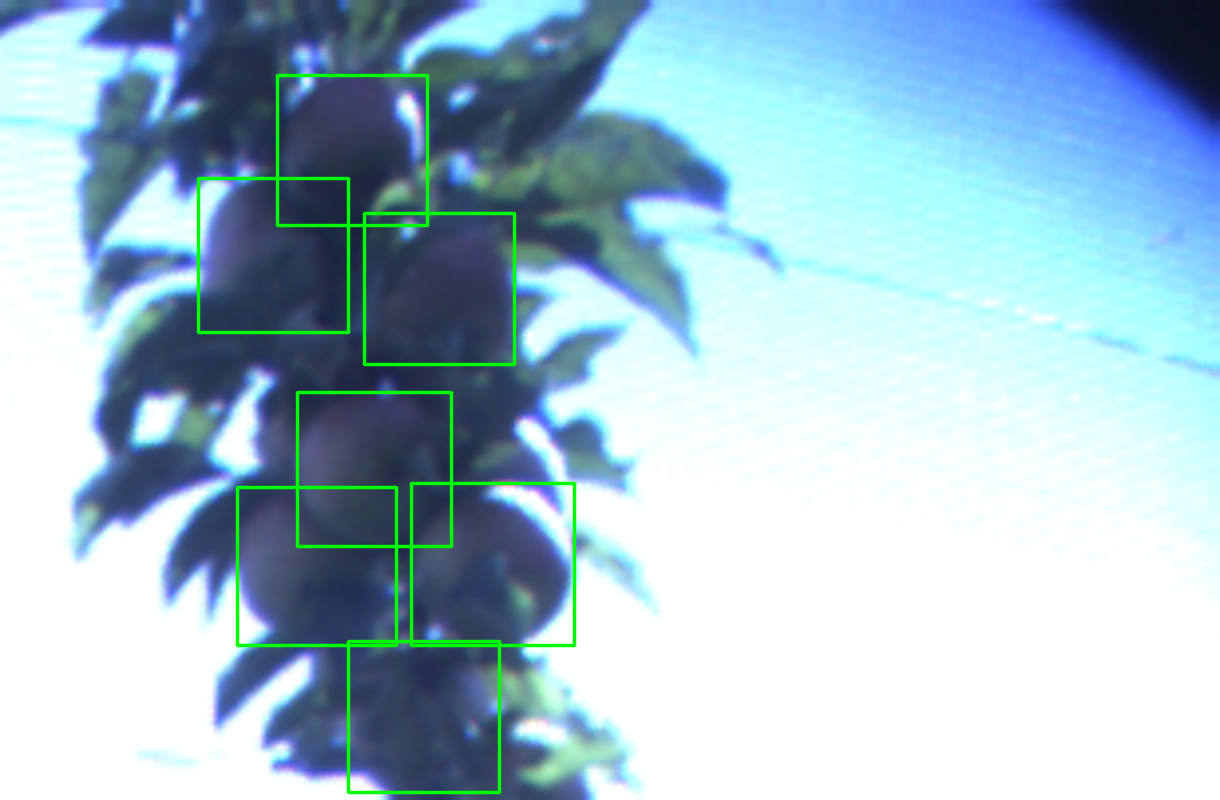
\includegraphics[width=0.31\textwidth]{figures/ch5/fig1_1.png}
    \label{fig1_1}
  }
  \subfigure[]{
    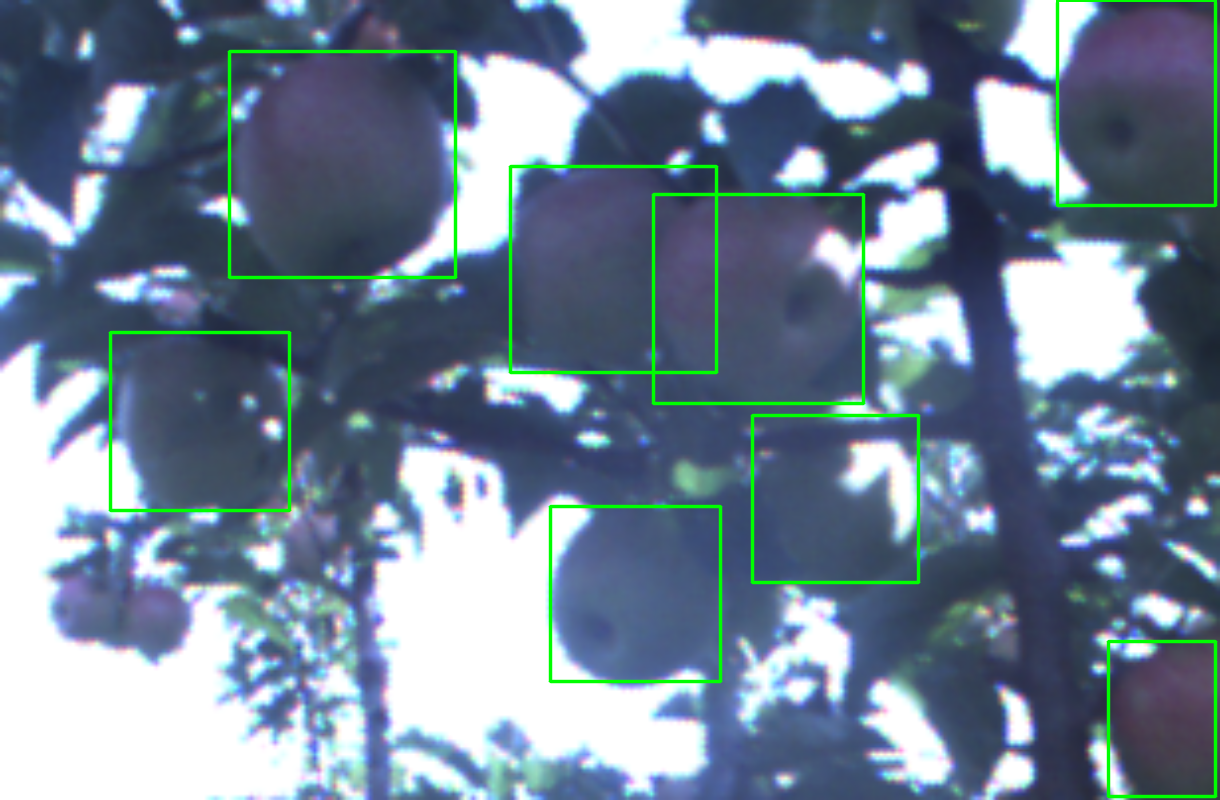
\includegraphics[width=0.31\textwidth]{figures/ch5/fig1_2.png}
    \label{fig1_2}
  }
  \subfigure[]{
    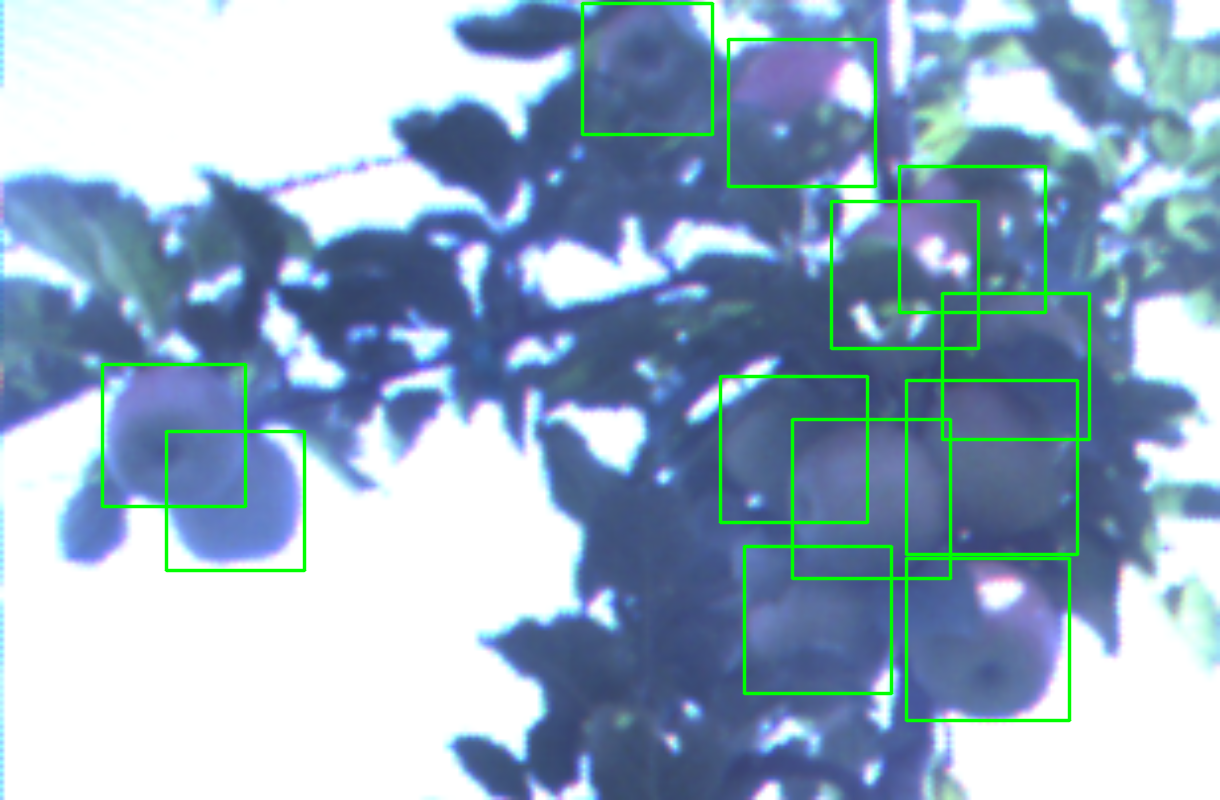
\includegraphics[width=0.31\textwidth]{figures/ch5/fig1_3.png}
    \label{fig1_3}
  }
  \caption{Cases of successful predictions: (a) in a tight fruit cluster, (b) between foreground and background fruits (bottom-left) and (c) in a fruit cluster with highly occluded instances. Green boxes represent true positive examples.}
  \label{fig1}
\end{figure}

 \begin{figure}[!ht]
  \centering
  \subfigure[]{
    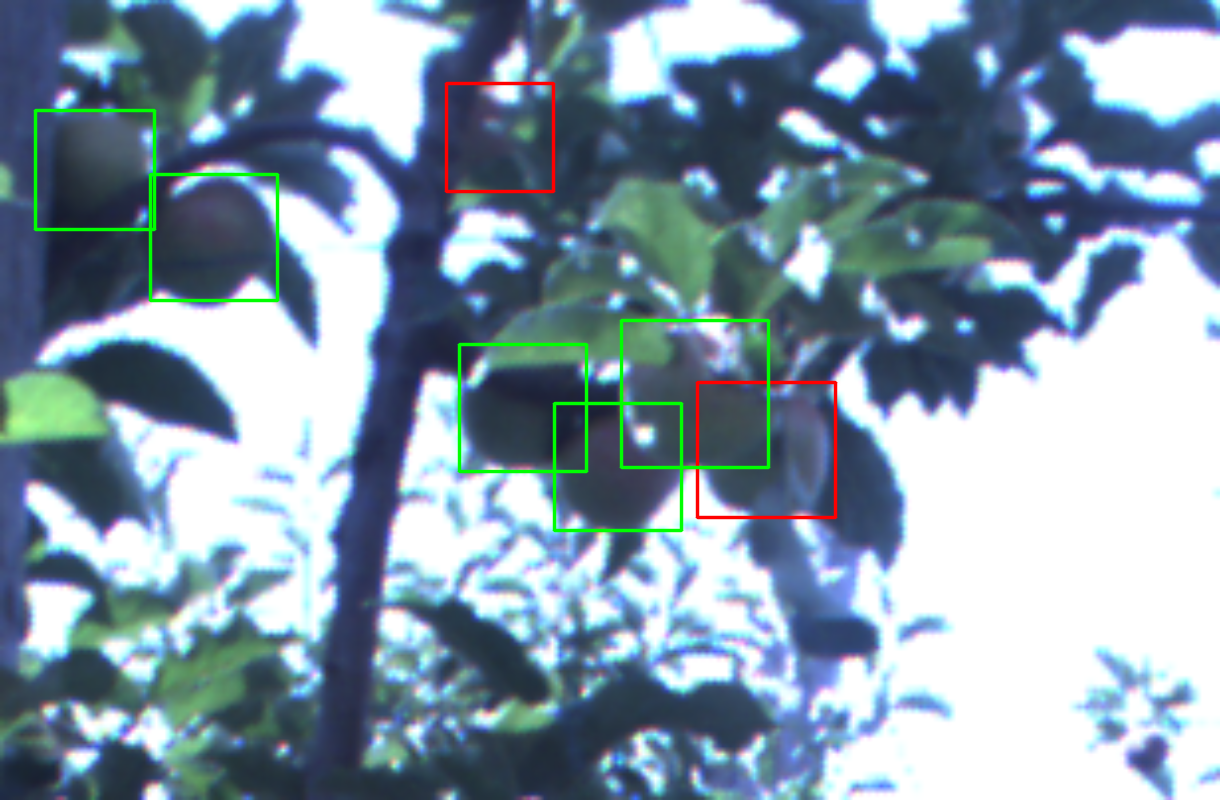
\includegraphics[width=0.31\textwidth]{figures/ch5/fig2_1.png}
    \label{fig2_1}
  }
  \subfigure[]{
    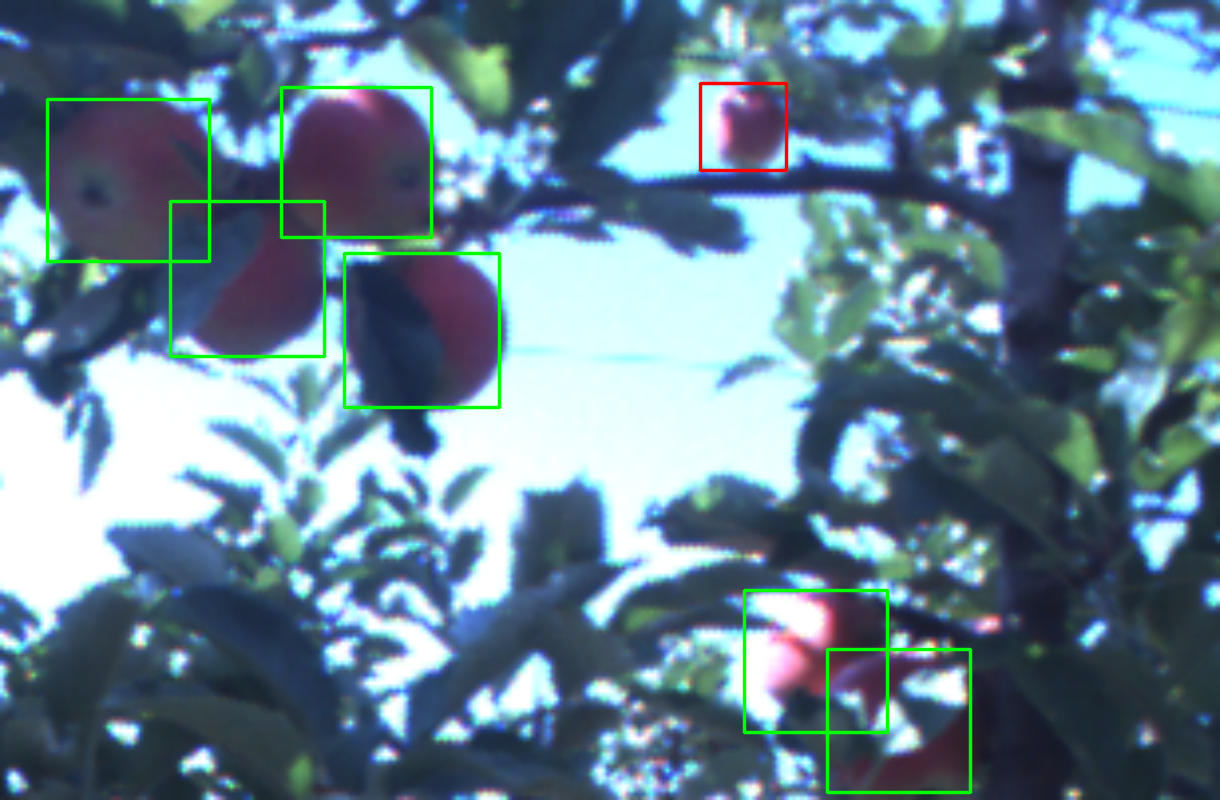
\includegraphics[width=0.31\textwidth]{figures/ch5/fig2_2.png}
    \label{fig2_2}
  }
  \subfigure[]{
    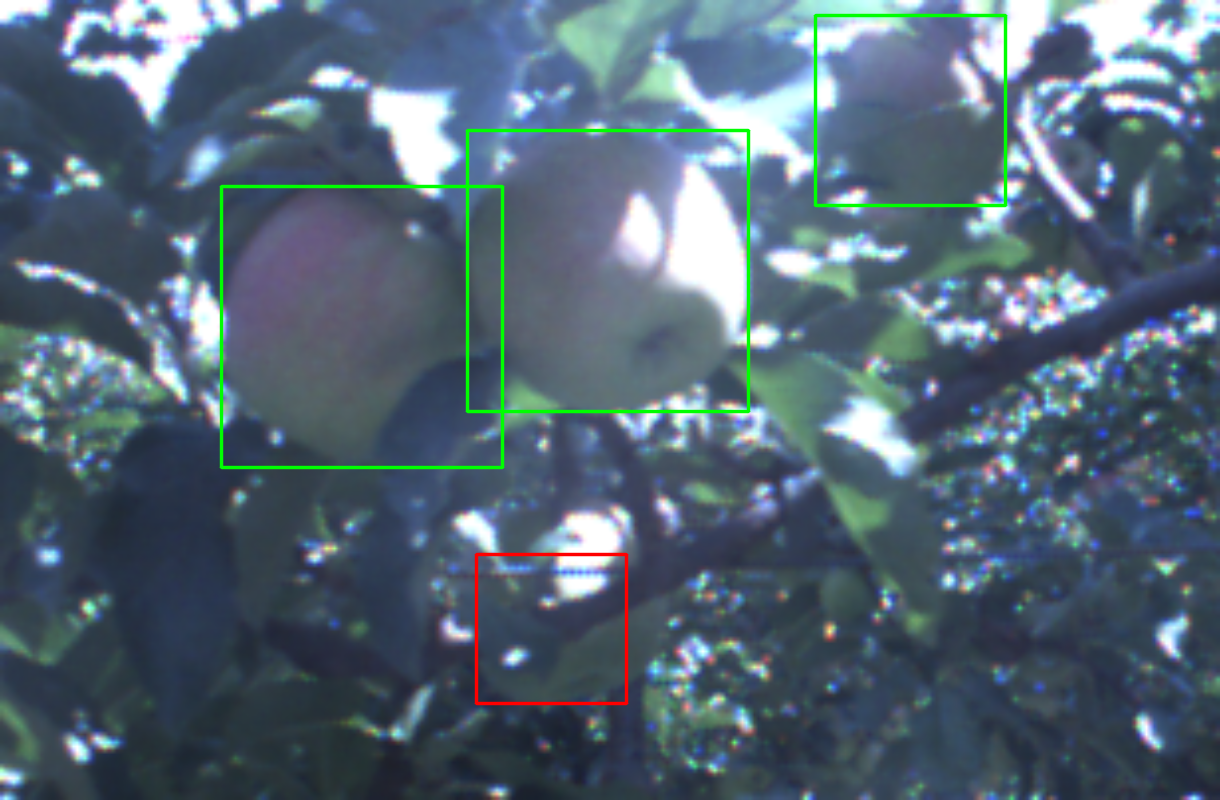
\includegraphics[width=0.31\textwidth]{figures/ch5/fig2_3.png}
    \label{fig2_3}
  }
  \caption{Error cases where apparently correct predictions are registered as false positives due to lack of annotation. Green and red boxes represent true and false positives respectively.}
  \label{fig2}
\end{figure}

 \begin{figure}[!ht]
  \centering
  \subfigure[]{
    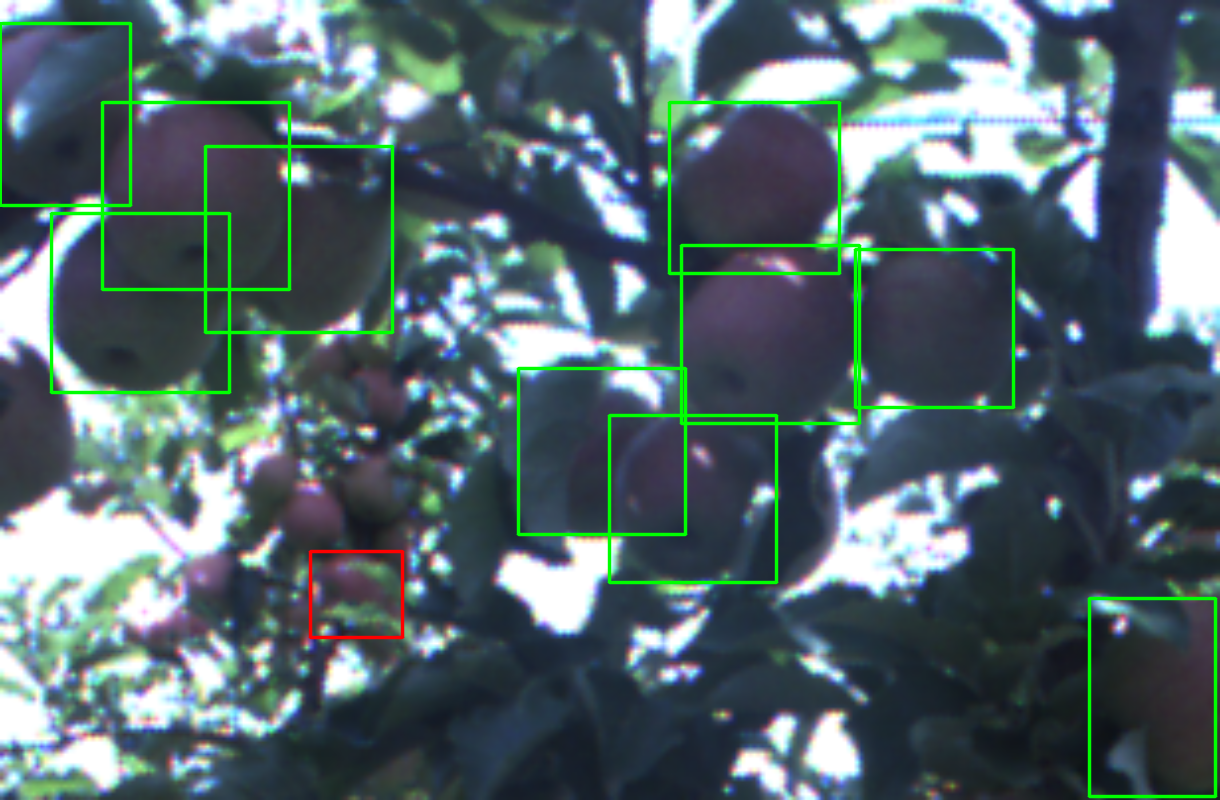
\includegraphics[width=0.31\textwidth]{figures/ch5/fig3_1.png}
    \label{fig3_1}
  }
  \subfigure[]{
    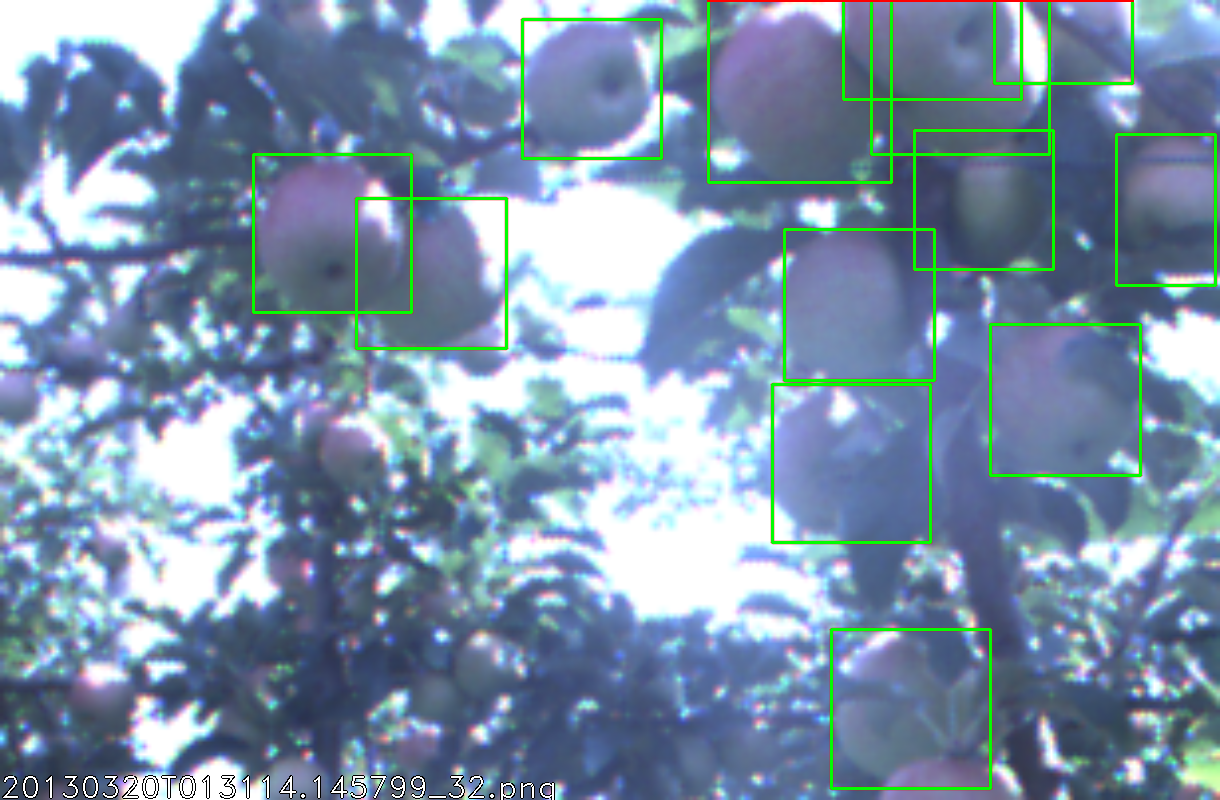
\includegraphics[width=0.31\textwidth]{figures/ch5/fig3_2.png}
    \label{fig3_2}
  }
  \subfigure[]{
    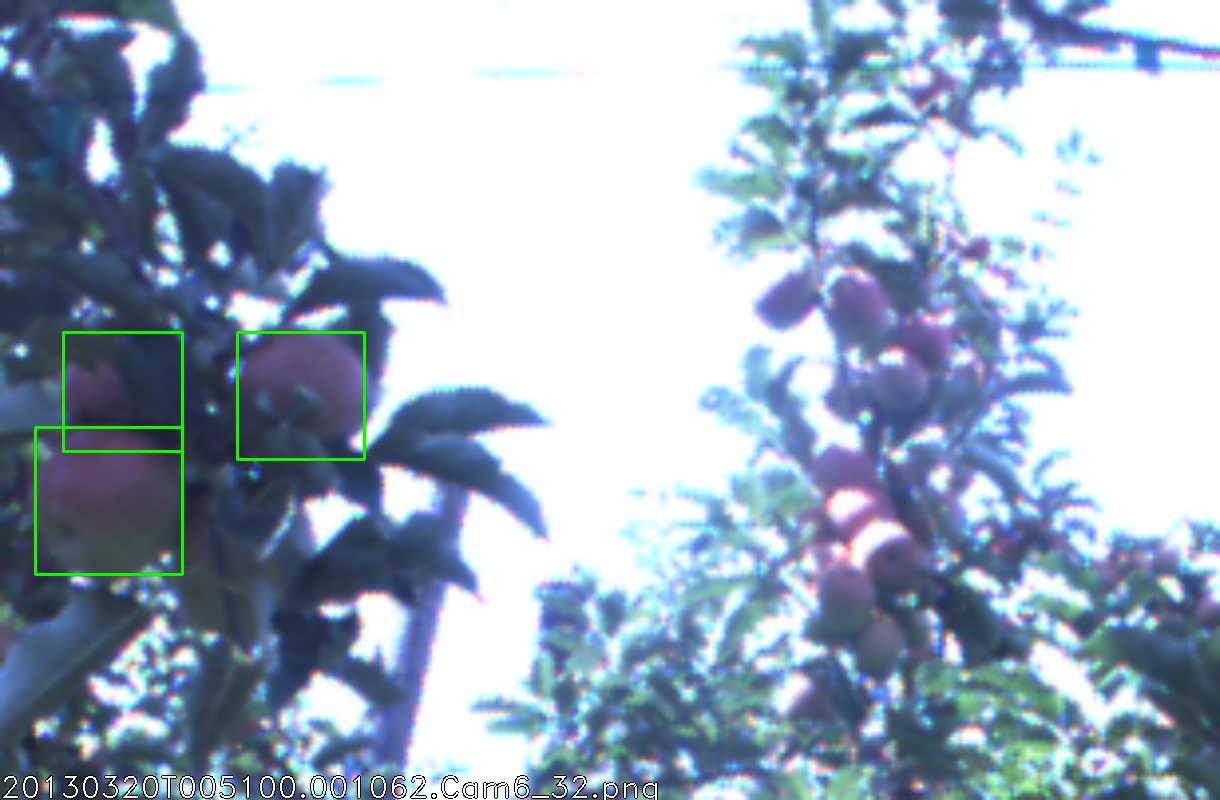
\includegraphics[width=0.31\textwidth]{figures/ch5/fig3_3.png}
    \label{fig3_3}
  }
  \caption{Some hard examples in the training dataset. The model encounters difficulties identifying relevant samples between foreground and background. If the model associates distance with the relative fruit size, this misleading rule indicates overfitting, as it does not apply in general. Green and red boxes represent true and false positives respectively.}
  \label{fig3}
\end{figure}

 \begin{figure}[!ht]
  \centering
  \subfigure[]{
    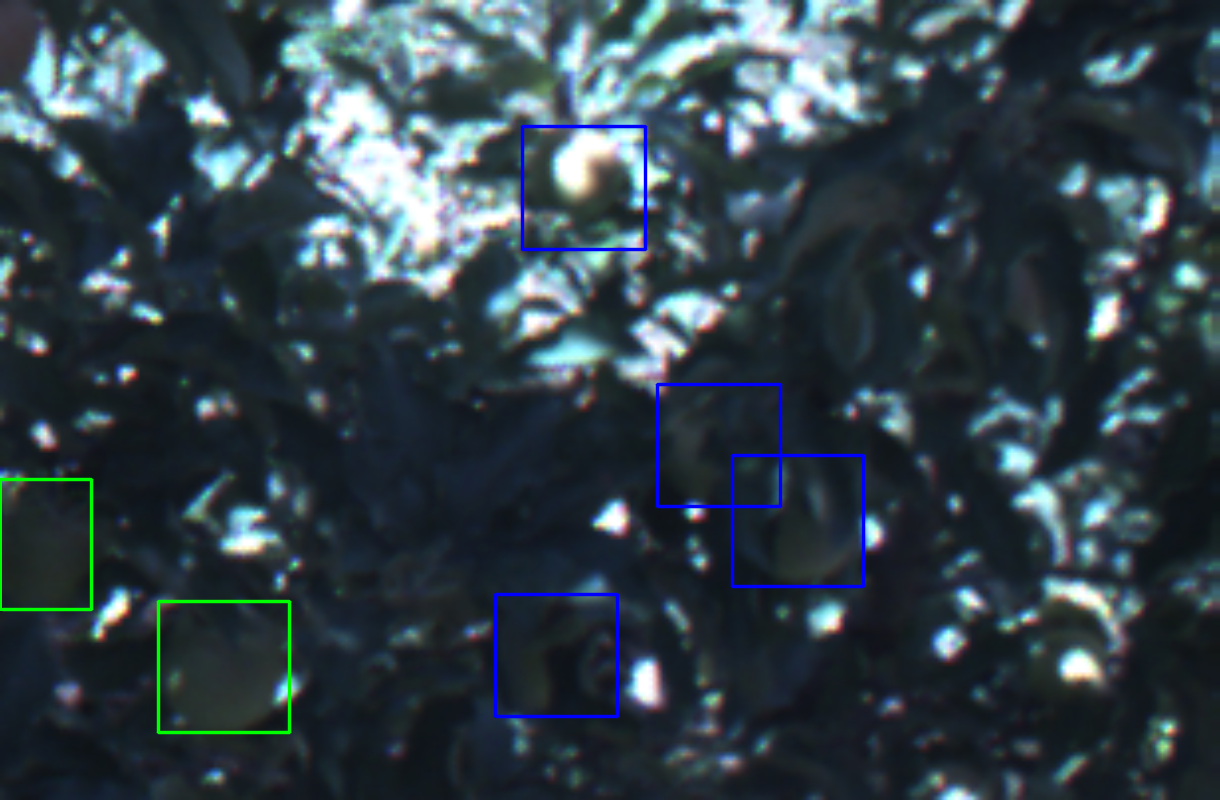
\includegraphics[width=0.31\textwidth]{figures/ch5/fig4_1.png}
    \label{fig4_1}
  }
  \subfigure[]{
    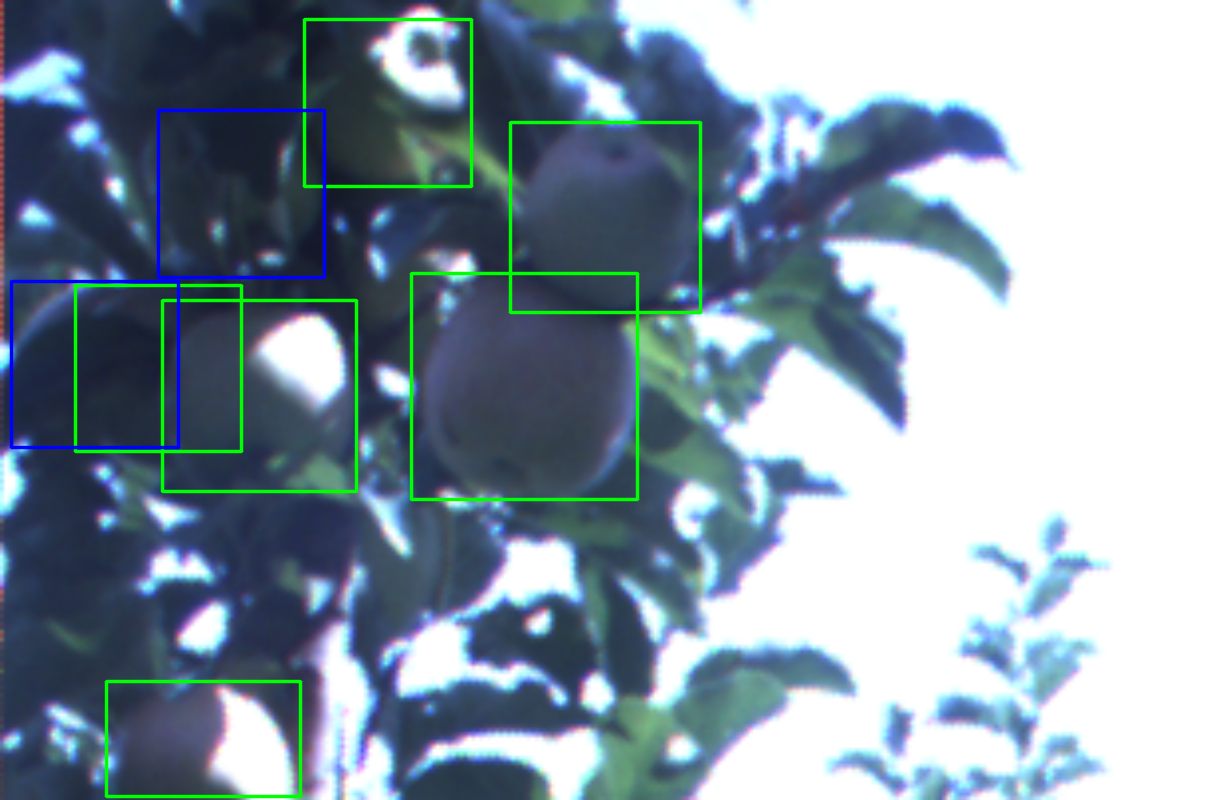
\includegraphics[width=0.31\textwidth]{figures/ch5/fig4_2.png}
    \label{fig4_2}
  }
  \subfigure[]{
    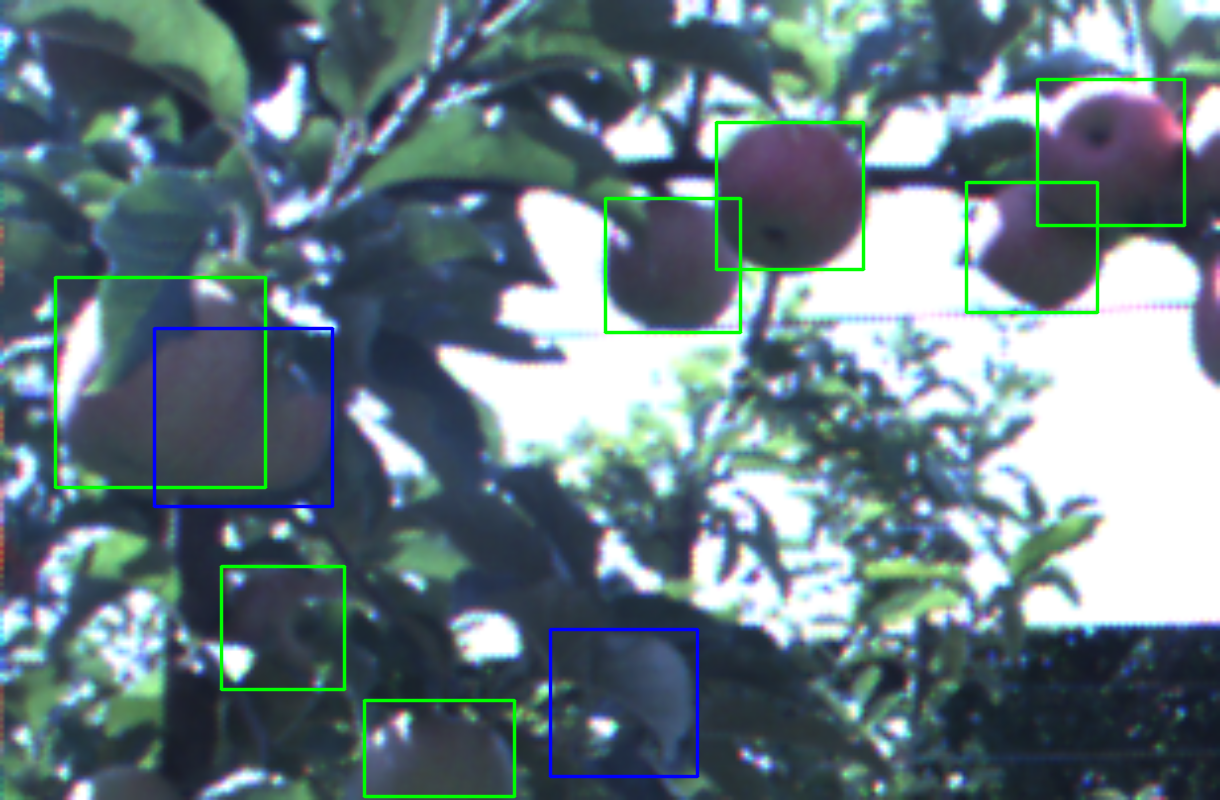
\includegraphics[width=0.31\textwidth]{figures/ch5/fig4_3.png}
    \label{fig4_3}
  }
  \caption{Interesting false negative predictions from the testing dataset. Errors due to: (a) illumination conditions, (b-c) dubious ground truths. In (b-c), it can be seen that occluded instances with $\text{IoU} \geq \text{NMS}_{th}$ are suppressed to avoid multiple detections of the same object.}
  \label{fig4}
\end{figure}

